%\documentclass[floatfix,11pt]{revtex4-1}
\documentclass[floatfix,11pt]{article}
\usepackage{color}
\usepackage{graphicx}
\usepackage{bm}
\usepackage{amsfonts}
\usepackage{mathrsfs}
\usepackage{amsmath}
\usepackage{amssymb}
\usepackage{setspace}
\usepackage{wrapfig}
\usepackage{fancyhdr}
\usepackage[labelfont=bf]{caption}
\usepackage{enumerate}
\usepackage{enumitem}
\usepackage{array}
\usepackage{natbib}
% \usepackage{pdfpages}
\newcolumntype{C}[1]{>{\centering\let\newline\\\arraybackslash\hspace{0pt}}m{#1}}

%----- Letter ----
\textwidth  = 6.5in
\textheight = 8.8in

\oddsidemargin = -0.in
\evensidemargin = 0.0in
\topmargin = -0.5in
\headheight = 0.5in
\headsep = 0.2in
\footskip = 0.4in

%%%%    HEADER     %%%%
\renewcommand{\headrulewidth}{0.75pt}
\pagestyle{fancyplain}
%\lhead{\small\textit{Mapping galaxies in spectral space}}
%\rhead{\small\textit{PI: Marina Meila}} 
\fancypagestyle{plain}

%%%%    FOOTER     %%%%
\renewcommand{\footrulewidth}{0.75pt}
\fancyfoot[LO]{\small\textit{DE-FOA-0002501}}
\fancyfoot[CO]{}
\fancyfoot[RO]{\small\textit{Page \thepage}}

%%%%%% my commands   %%%%%%


\newcommand{\dist}{{\rm dist}}
\newcommand{\epsi}{\varepsilon}
\newcommand{\D}{D}
\newcommand{\tily}{\tilde{y}}
\newcommand{\yg}{y_g}
\newcommand{\ygp}{y_{g'}}
\newcommand{\xg}{x_g}
\newcommand{\xgtrue}{x_{g}^{true}}
\newcommand{\xgptrue}{x_{g'}^{true}}
\newcommand{\xgf}{x_{g,l}}
\newcommand{\xgpf}{x_{g',l}}
\newcommand{\xgp}{x_{g'}}
\newcommand{\sigg}{\sigma_g}
\newcommand{\siggf}{\sigma_{g,l}}
\newcommand{\siggp}{\sigma_{g'}}
\newcommand{\siggpf}{\sigma_{g',l}}

\newcommand{\ml}{ML}
\newcommand{\sklearn}{{\tt scikit-learn}}
\newcommand{\mmani}{{\tt megaman}}
\newcommand{\gmani}{{\tt GigaMan}}

\newcommand{\comment}[1]{}
\newcommand{\mmp}[1]{\textcolor{blue}{MMP:#1}}
\newcommand{\bit}{\begin{itemize}}
\newcommand{\eit}{\end{itemize}}


\begin{document}
\begin{center}
{\sc Title} Vertical leap: Embedding high-dimensional data with functional analysis/consistency theorems and super-computers

\textbf{PI: Marina Meila} Professor of Statistics

University of Washington
% Department of Statistics, Box 354322, Seattle WA 98195-4322, 

Phone: 206-543-8484,  {\tt mmp@stat.washington.edu}

{\textbf DE-FOA-0002501}

\line(1,0){480}
\end{center}
\singlespacing
\vspace{-.75cm}
\noindent\begin{tabular}{lll}
\multicolumn{3}{c}{Some examples of data reduction}\\
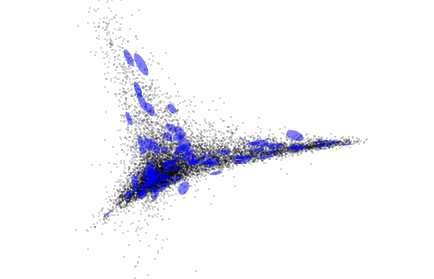
\includegraphics[width=2.1in]{Figures/word2vec_rmetric_plot_noaxis_trim.png} &
%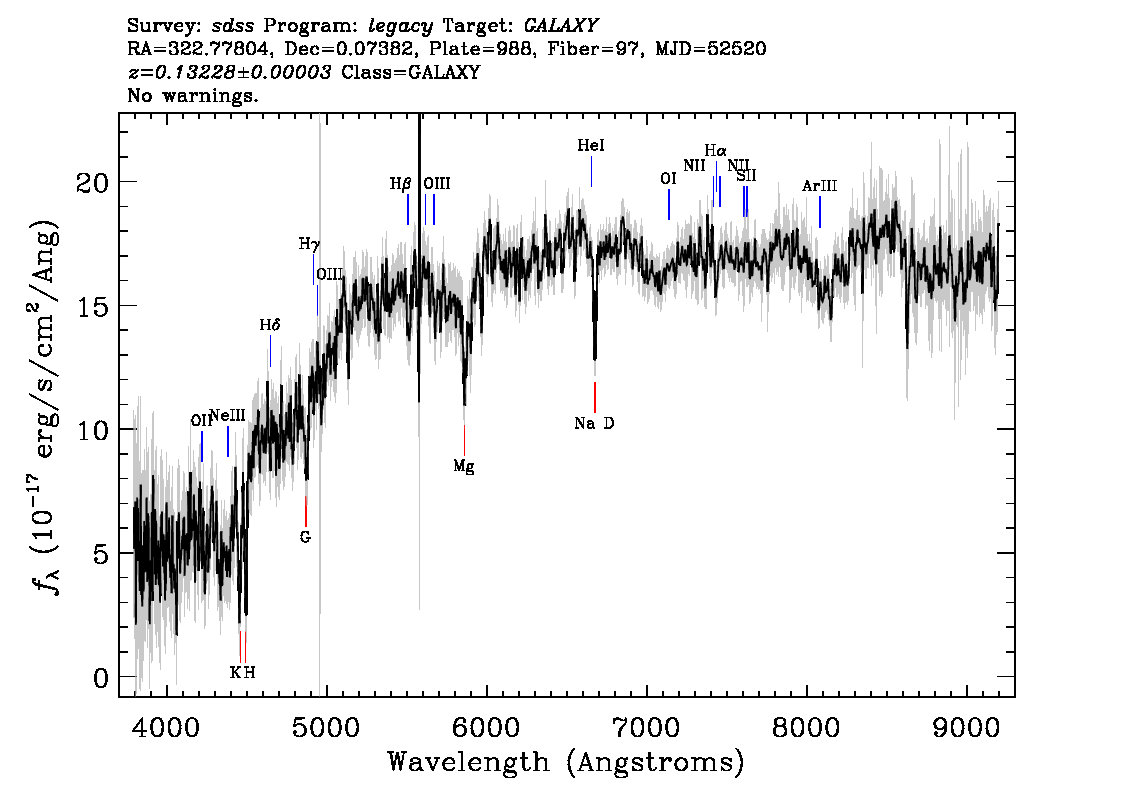
\includegraphics[width=2.2in]{Figures/specById_asp.png} & 
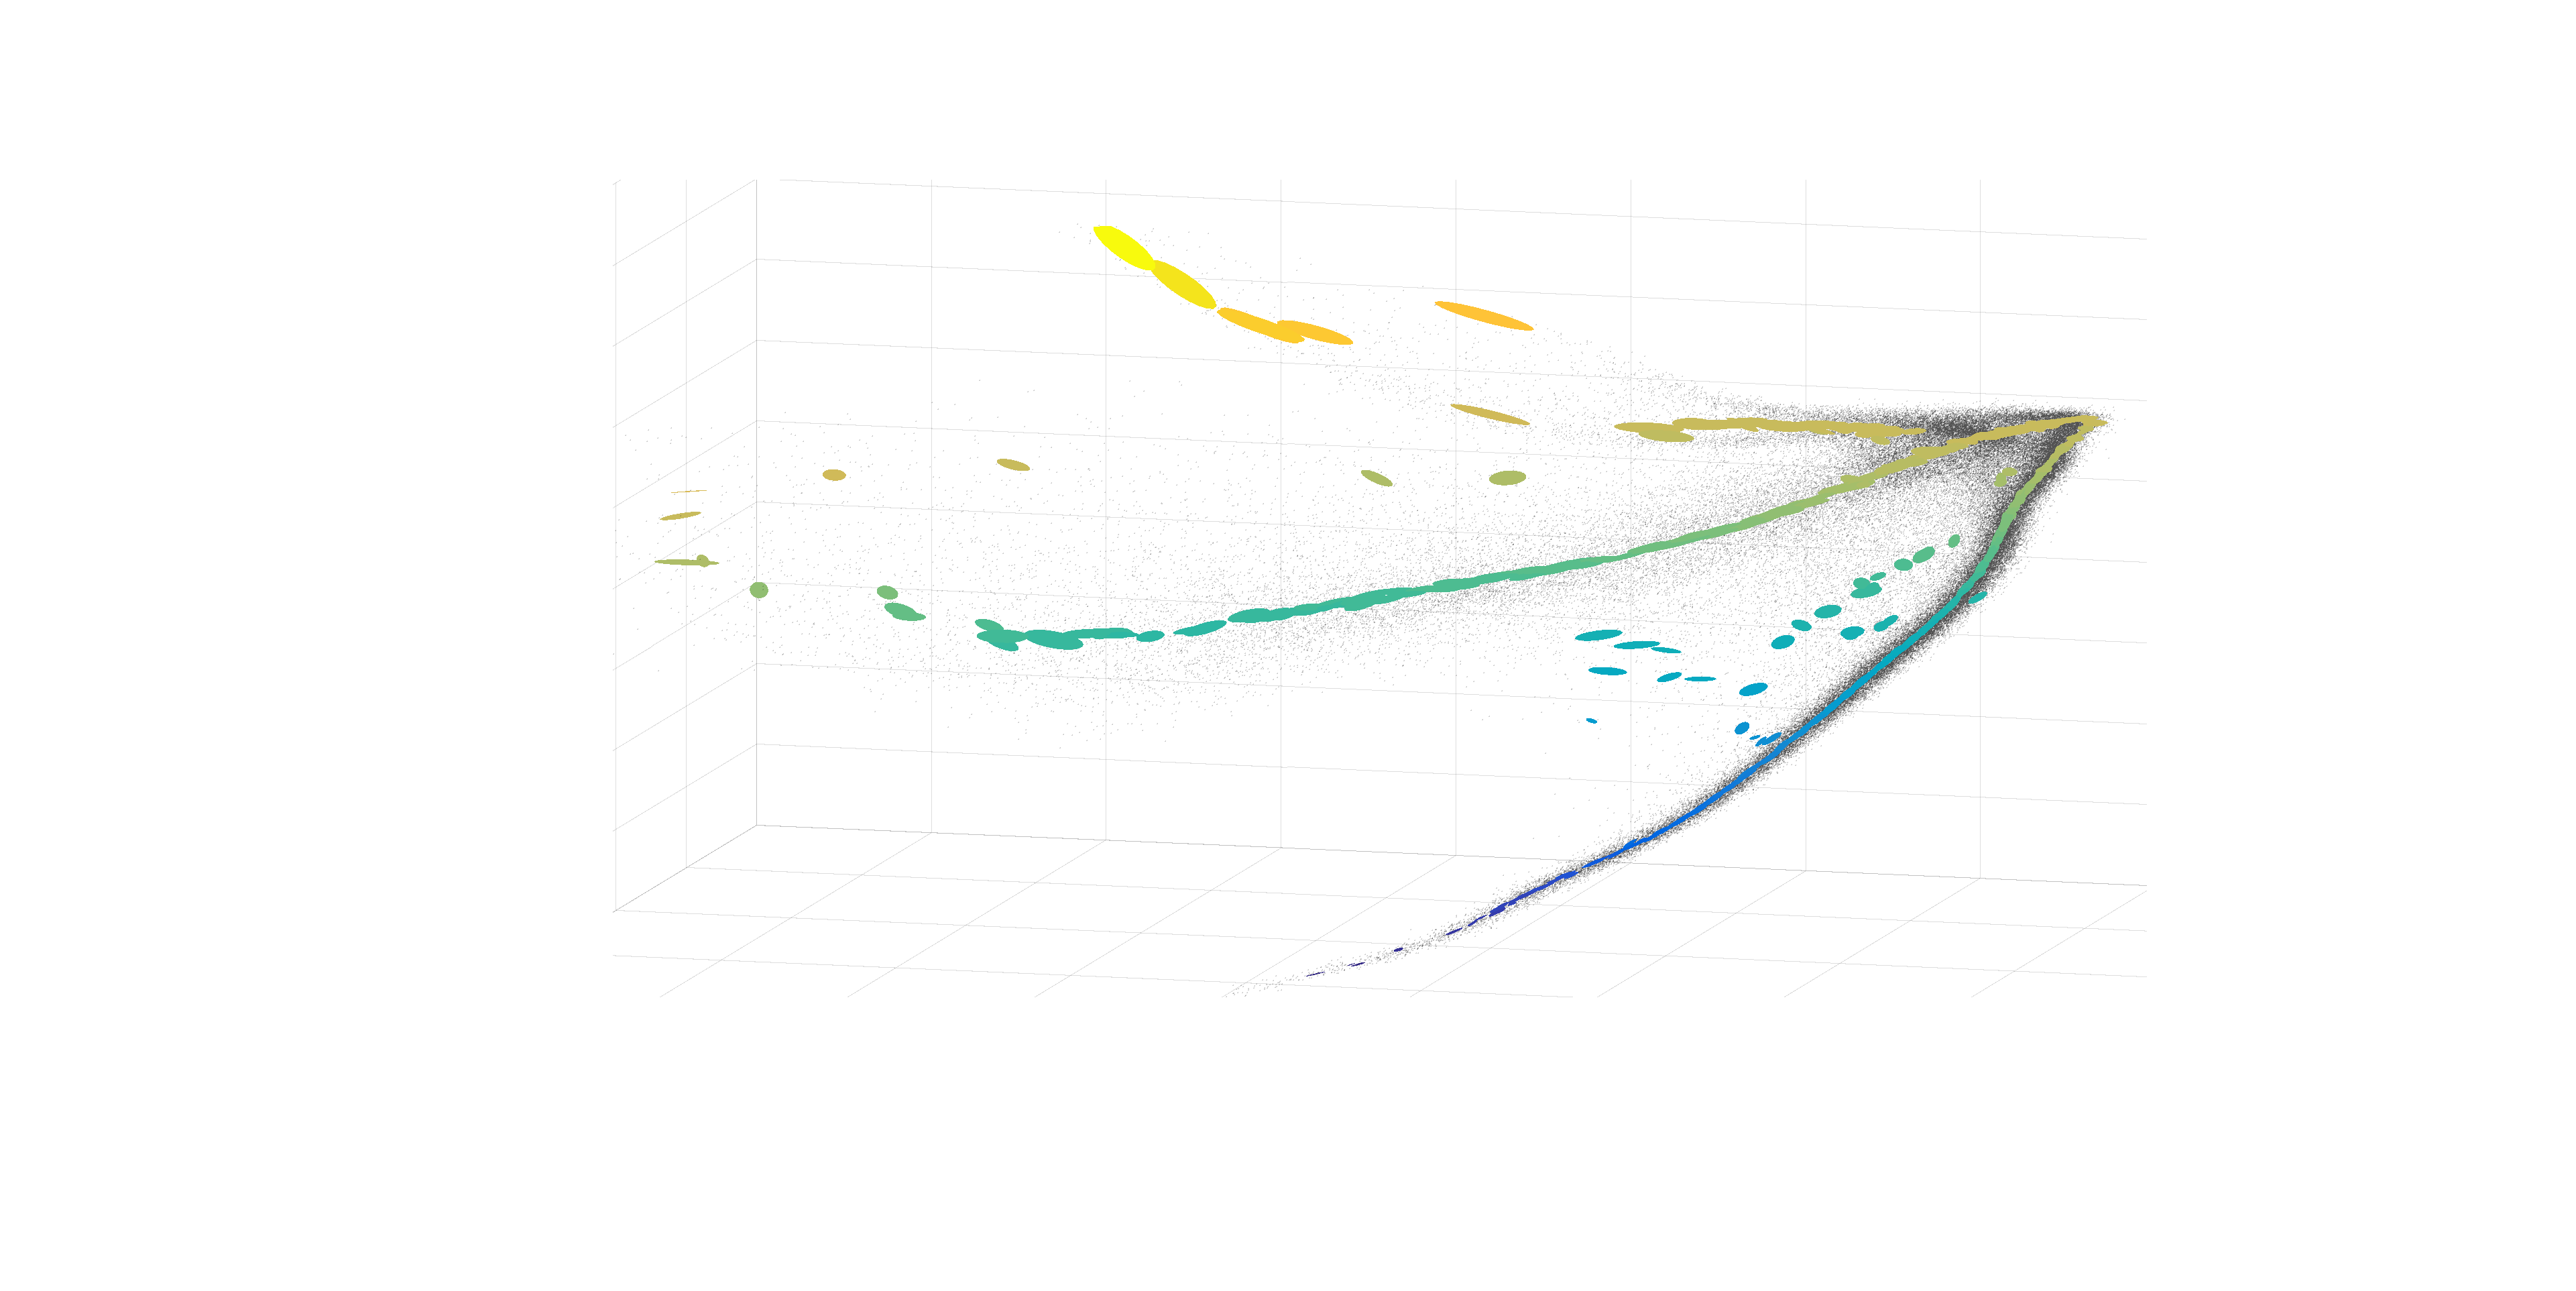
\includegraphics[width=2.5in,clip=]{Figures/spectrum_data_before-trim.pdf} 
&
\includegraphics[width=2.5in,clip=]{Figures/smoothed_velocity_field_alpha_50.pdf}\\
\parbox[t]{2.1in}{3D embedding of 3,000,000 words and phrases represented in 300 dimensions from {\tt https://code.google.com/archive/p/word2vec/}}
&
\parbox{2.1in}{3D embedding of 675,000 spectra of galaxies from {\tt www.sdss.org} with 3750 wavelengths}
&
\parbox{2.5in}{Smoothed velocity field of 20,000 ocean buoys from {\tt
https://www.ndbc.noaa.gov}}
\\
\end{tabular}
\begin{tabular}{llll}
\multicolumn{3}{c}{Naive embedding algorithms introduce artefacts}
&
Measuring embedding distortion
\\
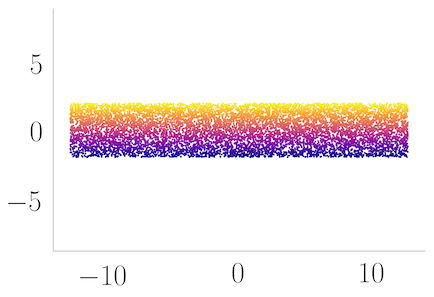
\includegraphics[width=1.9in]{Figures/D1_original_data.png} &
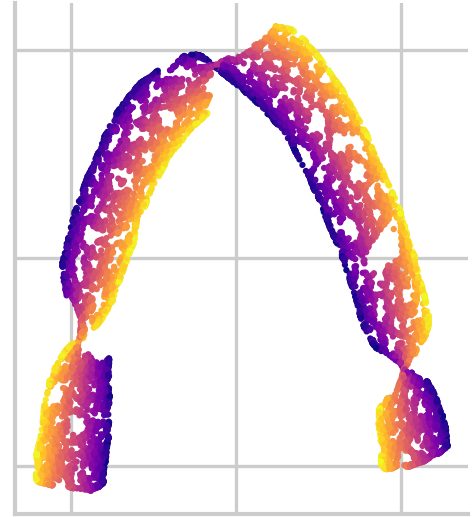
\includegraphics[width=1.in]{Figures/umap_mindist_comp.png} &
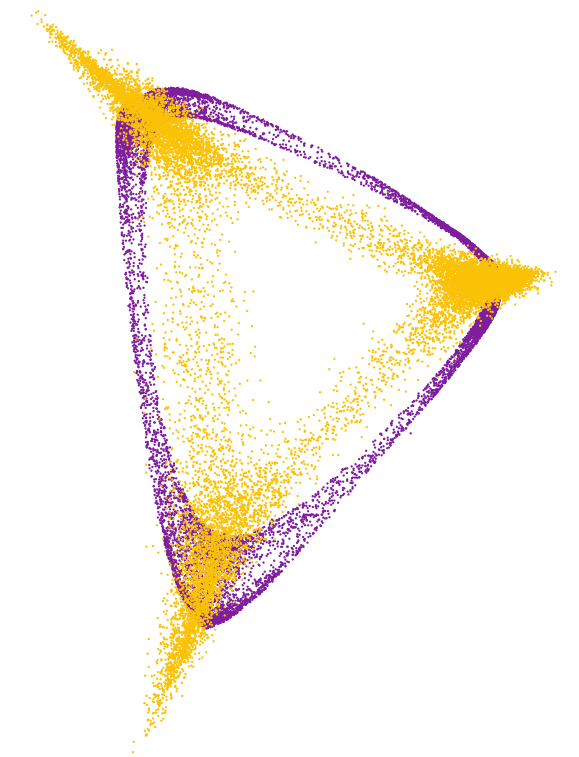
\includegraphics[width=1.3in,angle=90]{Figures/geometric_vs_normalized.png}
&
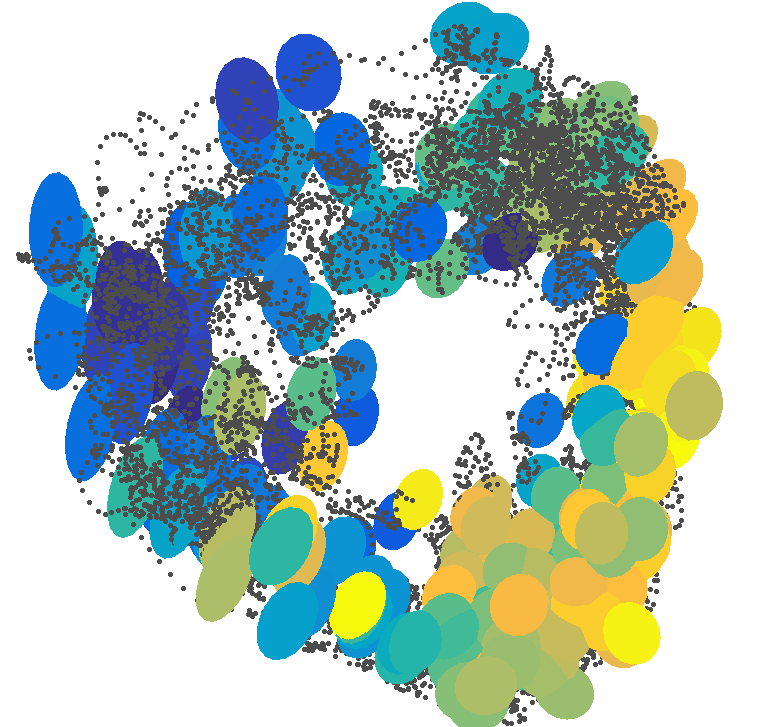
\includegraphics[width=1.3in]{Figures/aspirin-postclu1-phi234Rmetric-tau22.png}
\\
\multicolumn{2}{l}{\parbox{3in}{Figure .: Embedding of a 2D strip by UMAP, showing 4 clusters}}
&
\parbox{2.1in}{Two embeddings of molecular configurations of ethanol; the original data is a torus.}\\
%\parbox{2.1in}{Figure .:
\end{tabular}
\\ What is proposed: \gmani, a non-linear dimension reduction toolbox
in python, that scales to data matrices of order $n\times p \sim
10^{12}$, which implements the state of the art in the mathematics and
statistics of high dimensional geometric learning.


\textbf{Motivation}
\bit
\item data reduction for the sciences must come with guarantees of
  reproducibility (e.g. outputs not sensitive to initialization of
  algorithm), stability (outputs not sensitive to variations in
  sample), as well as with rigurous methods to quantify the loss of
  information and the variability of the result, and with
  guarantees of preserving desired properties/features/(geometric)
  characteristics
\item here we are concerned with data in the form of high-dimensional points, such as spectra of galaxies (dim = number of spectral bands, but not quite), spatial locations of the atoms in a molecule (dim = number atoms $\times$ spatial dimension 2 or 3), state space of a dynamical system, as well as with non-vector data for which a {\em distance} between points can be defined, such as biological sequences, words and phrases, job descriptions, images, etc.
\item data reduction consists primarily of dimension reduction, since a very large number of high dimensional data are described by a much smaller number of degrees of freedom (for example, while image resolution can grow from Mega-pixels into Giga-, the image contens does not become richer at the same rate)
\item but non-linear embeddings can provide data reduction in other ways too. Smoothing the data, by projecting it onto a local manifold. Subsampling the regions where the data is too dense. More about advantages of subsampling.
  \eit
  What we will do, again.

  \textbf{Challenges}
  \bit
\item Estimating non-linear geometry from ``point cloud'' data is very hard statistically and mathematically. Because of the non-linearity of the space, e.g.  (variable) local curvature, naive methods of dimension reduction end up being biased or even inconsistent (tending to unreasonable/degenerate limits when $n\rightarrow \infty$. ``Errors don't average to 0'' in non-linear geometric estimation. The statistical and mathematical methods needed to analyze the properties of embedding algorithms and to design consistent, unbiased, ones are highly technical, and are a field under development. [Proof that of the most popular methods LLE, t-SNE, UMAP are unstable and inconsistent in the limit, depend on parameters that must be set by eyeballing]
\item Math is too highly technical to be read by most scientists, engineers and computer scientists. This is a barrier to the adoption of the state of the art knowledge. 
\item Embedding algorithms relie on a form of interpolation between neighbors (are similar to kernel density estimation). Finding neighbors in high dimensions and large data sets is the main computational bottleneck. 
\item Eigendecompositions is the {\em perceived} bottleneck, but the PI's own experience and communications with experts show that with careful/expert reweighing, preprocessing, the eigendecomposition step is more tractable than the nearest neighbor step. In particular, eigendecomposition does not depend on the data dimension $p$, but only on the sample size $n$. 
\item Even if phenomena well approximated by manifolds, in fact they are multiscale (or equivalently, noise has structure, is not i.i.d. and not isotropic), and rarely is the dimension constant. One of the contributions of this proposal is to rigurously develop embedding methods with variable dimension (unions of manifold, stratified spaces)
\item What if data can't be stored in memory? Distributed data? I'd rather not deal with it now. We'll see. 
  \eit
  
  {\bf Why non-lin dim reduction great for scientific data}
  \bit
  \item Often data
dimension is a function of the resolution of the instrument and does
only slowly add new degrees of freedom. Hence, higher $p$ means
sharper measurements, less instrument noise: good. Highly non-uniform
sampling (e.g. molecular configurations are subject to Boltzmann
distribution, with exponential variations of density). When data
non-uniform, in highly concentrated regions it becomes redundant --
only a freaction of it is sufficient to estimate the geometry;
statistically, subsampling the data in this regime produces a faster
converging embedding.
\item many physical processes described mathematically by manifolds and vector fields. hence the data driven approximations have a basis for being supported by physical theory.
\eit

{\bf What we will do}
\bit
\item Design implementable algorithm for approximate fast nearest neighbor method based on theoretical state of the art. Main sources Indyk, Charikar, Razenshteyn. MM
\item Proof that {\em this} approximate nearest neighbor is sufficient to assure convergence when used with manifold learning algorithms Source: Fefferman et collabs\footnote{Fefferman is Fields medalist.} MMM
\item The methods above depend on constants with undknown values. Design methods to estimate the constants from data (e.g. a form of CV, by geometric consistency, etc). MMM
\item Summarizing/subsampling big data: Coresets and hierachical indexing. Sources TBW. M 
\item Translate the methods above into algorithms. M
\item Implement the algorithms efficiently to obtain a toolbox of neighborhood construction algorithms, and a toolbox of embedding algorithms. These will be called the core algorithms. M
\item Develop around the core algorithms a suite of other methods.
 \bit
 \item Preprocessing: subsampling, estimating the local neighborhood size, estimating the intrinsic dimension, data indexing (related to subsampling) M
 \item Non-embedding methods based on neighborhood graphs: L1 Laplacian and Helmholtz-Hodge decomposition, other TDA applications, kernel regression on manifolds M
 \item Postprocessing: estimating/correcting the embedding by metric learning and Riemannian Relaxation, estimating the noise (e.g. MSE, locally), stratifying the data by dimension, MM
   \eit
 \item Data reduction for chemistry and materials sciences
 \item Data reduction for astronomy 
   \bit
 \item LSST
 \item simulated data
   \eit
 \eit


\underline{\bf Team expertise} Team of exceptional depth and breadth.
MMP has spent more than 10 years pondering the problems in non-parametric data analysis and geometric learning. She is aware of of the theoretical advances, and capable to discern their significance w.r.t. practical problems and existing data. More specifically, theorems must relie on testable assumptions to be of methodological value. The PI's contribution is focused on this aspect: how to make mathematics meet real life problems? What can we measure from real data so that we can guarantee that theory applies?
The PI is an expert in Machine Learning, and has a long track record of developing algorithms in geometric data analysis and unsupervised learning, and of deploying them as software packages.

All team members are long term collaborators, and all are Senior Fellows of the eSCience Institute. Meila, Connolly and Ivezic collaborated on more than five grant proposals; Meila and Beck collaborated on four grant proposals, two of them funded by the DE under FOA .... Meila and Vasquez-Mayagoitia collaborated on the ALCF Grant .... As part of this collaboration, the software \mmani~was ported on the Theta, and UW student Yu-chia Chen visited ALCF. \mmani~originated in the first Data Science Incubator as a collaboration between Meila and Jake VanderPlas. 

%The PI is in the unique position to be aware of the theoretical advances in manifold learning and geometric data analysis, 


%brings extensive experience in ML, from the statistical issues \cite{PerraultMMcQueen:nips17} to software \cite{mcqueenMVdpZ:megaman16,*mcqueenMVdpZ:megaman-jmlr16}


{\bf Previous work}

{\bf Existing support} No other funding exists for this project. collaborative grant of 170M CPU hours at the Argonne Labs Computing Facility (see CV) since September 2017 for the PI's research on manifold learning in chemistry.

{\bf Readiness} The package {\tt megaman}\footnote{{\tt http://mmp2.github.io/megaman}} \cite{mcqueenMVdpZ:megaman16,*mcqueenMVdpZ:megaman-jmlr16} implements all the manifold learning algorithms described in this proposal. Our pilot experiments (one shown in Fig. 3) and \cite{Yip04} \comment{prove that that we have the computing resources and }strongly suggest that low dimensional structure exists in the SDSS data. The PI and co-PI are co-mentoring PhD student Yu-chia Chen, and are committed to developing open source machine learning software (e.g {\tt megaman}, contributions to {\tt scikit-learn}). \comment{With infrastructure and collaboration in place, we}We request funding for one graduate student, and one undergraduate student (only computing costs) for 12 months.


{\bf Timeline} 

\vspace{-2.1em}
\bibliographystyle{abbrv}
\bibliography{proposal,SDSS_LLE}

\vspace{0.6em}

%https://www.alcf.anl.gov/projects/constructing-and-navigating-polymorphic-landscapes-molecular-crystals

\vspace{0.6em}

\newpage
\centerline{\textbf{Senior Personnel}}
\begin{tabular}{llll}
  Last name & First name & Title & Institution\\
  \hline
Meila & Marina & Professor & University of Washington\\
Beck & David & Professor &  University of Washington\\
Ivezic & Zeljko & Professor &  University of Washington \\
Connolly & Andrew & Professor &  University of Washington (???)\\
Juric & Mario & Associate Professor &  University of Washington (???)\\
Vasquez-Mayagoitia & Alvaro & Computational Scientist & Argonne National Computing Facility\\
\end{tabular}

\centerline{\textbf{Collaborators, Co-editors, and Graduate and Postdoctoral Advisors and Advisees of the PI and Senior/Key Personnel}}
\begin{tabular}{llll}

\end{tabular}

\end{document}
I am proposing to expand my geometric learning package megaman to
bigger data and to include procedures coming from the newest math and
theoretical stats research on geometric data analysis in high
dims. The heavy lifting will be 2/3 in the math/stat part, surprising
as it seems, because the methods that have guarantees, the stuff that
only theorists and I know of, is very abstract, and is proven to work
only on paper. There are 2-3 bottlenecks of this kind. The rest would
be dominated by applications, with implementation being split between
"theory" and "app", the way I see it now.


DOE has issued this solicitation. Pre-proposal on May 4, but UW has an
internal competition with deadline a week earlier. Would you like to be
key personnel on this? There will be no funding for our collaboration (see
the budgets are very small) but it may lead to something bigger. I want to
propose to expand megaman to bigger data and to include procedures coming
from the newest math and theoretical stats research.


I am proposing to expand megaman (my manifold learning/geometric learning
sofware) to bigger data and to include procedures coming from the newest
math and theoretical stats research on geometric data analysis in high
dims.

bigger: now megaman handles 10^6 points x 1000 dimensions. I would scale
it to 10^12 points x dimensions or bigger.
I have invited a collaborator from ALCS (Argonne labs) who is into exa
scale computing, and I would like to also invite 1-2 colleagues from Chem
Eng.

Part 2: if this isn't the right thing for you, but if you are interested
in dimension reduction for large data sets, let's write a NSF proposal
some time. I have material from a previous proposal that was funded at 50%
level, and I can reuse the remaining 50% of what I wanted to do.

Let's reply in some random order:
-- never tried on 20K dimensions but I don't see why it would not work if scikit learn worked. megaman was written with Jake VdP so it inherits the API, it's public, and it's listed by the ASCL too. if your daughter gets something done with it I'd love to showcase it (e.g. get a picture and a caption for the web page). my student Sam can help with the installation.

https://sites.stat.washington.edu/mmp/software.html

-- the MN model is a great one. if you are interested in something bigger and science like, i'll send you some stuff in a few days about the things I've been doing and planning to do.

-- I'm not too worried about getting to 10^9 points. In 2015 we got to 10^6 by just doing the sensible thing, nothing else. An I've had 6 years to learn more about all levels of the problem, from the math to supercomputers. and all levels are getting faster. memory management will be the hardest part probably. i can of course tell you about other bottlenecks and if the pre-proposal gets approved i'll write about them very soon. 

-- this proposal: the estimated award size is 150K/year (they are funding mathematicians:) and I do need to fund 1 student x 4q from it to do all the math and statistics and I also hope that Jim Pfaendtner and maybe David Beck will be involved. So, of course I would like Andy and Mario but I want to make sure they know that the financial returns will be modest. This said, it would be fantastic to work together again. 

(fresh good  news, my collaborator from Argonne is on board!)

Did I reply to everything? hope so. Glad to hear so many news from you! 

Marina

On 4/21/21, 9:40 AM, "Zeljko Ivezic" <ivezic@uw.edu> wrote:

             Hi Marina,
long time no see! I hope you and family are well in these crazy times.

We (Andy, Mario, me) are working with SLAC on a similar DOE proposal
but I think it’s a different call.

I am very interested in manifold learning and dimensionality reduction
because of LSST. Please let me know if I can help you with anything.
Eventually, I’d like to learn more about how you plan to scale megaman
up by a factor of million (!), as well as to discuss a possible NSF proposal.
Just a few days ago, I gave a colloquium at MN astrophysics and talked
with colleagues there about their program that combines astronomy and
statistics (funded by NSF). Their model is to have two students, one from
astro and one from stats, approach the same problem, and have two
mentors, one from astro and one from stats. After two years, they are
very happy with how this concept works in practice.

Please let me know if you want me to include Andy and Mario. Andy moved
on to become e-Science Director, and Mario took over as DiRAC Director.
          Cheers, Zeljko

PS
Can your megaman do 25,000 points with 20,000 dimensions? I am asking
for my daughter - she’s finishing her term project and that is her data set from
biology context. She’s used LLE and the classification results are encouraging
but not perfect (she also has labels for 30 classes from an independent work).
Actually, I don’t even know if megaman is in public domain.
